\documentclass[border=5pt]{standalone}
\usepackage{tikz}
\usepackage{xcolor}
\usetikzlibrary{calc,shadows.blur}

% J5 - Beige hollow cylinder (tube)
\begin{document}
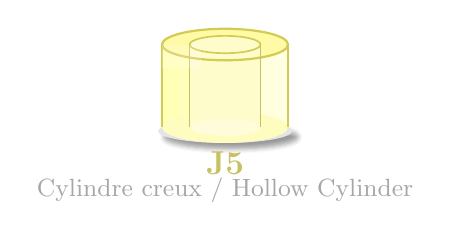
\begin{tikzpicture}

% Shadow
\fill[gray!20,blur shadow={shadow blur steps=5}] (0,-0.6) ellipse (0.85 and 0.15);

% Outer cylinder side wall
\fill[left color=yellow!30!white, right color=yellow!10!white, middle color=yellow!20!white]
  (-0.8,-0.55) rectangle (0.8,0.5);

% Bottom ellipse outer
\fill[yellow!25!white] (0,-0.55) ellipse (0.8 and 0.2);
% Bottom ellipse inner hole
\fill[yellow!15!white] (0,-0.55) ellipse (0.45 and 0.11);

% Top face outer
\fill[yellow!35!white] (0,0.5) ellipse (0.8 and 0.2);
% Top face inner hole
\fill[white] (0,0.5) ellipse (0.45 and 0.11);

% Inner tube wall (visible through hole)
\fill[yellow!20!white]
  (-0.45,-0.55) -- (-0.45,0.5)
  arc[start angle=180,end angle=0,x radius=0.45,y radius=0.11]
  -- (0.45,-0.55)
  arc[start angle=0,end angle=180,x radius=0.45,y radius=0.11];

% Outlines
\draw[yellow!60!gray, line width=0.8pt] (0,0.5) ellipse (0.8 and 0.2);
\draw[yellow!60!gray, line width=0.6pt] (0,0.5) ellipse (0.45 and 0.11);
\draw[yellow!60!gray, line width=0.8pt] (-0.8,-0.55)--(-0.8,0.5);
\draw[yellow!60!gray, line width=0.8pt] (0.8,-0.55)--(0.8,0.5);
\draw[yellow!50!gray, line width=0.6pt] (-0.45,-0.55)--(-0.45,0.5);
\draw[yellow!50!gray, line width=0.6pt] (0.45,-0.55)--(0.45,0.5);

% Highlight
\fill[white,opacity=0.2] (-0.8,0.2) rectangle (-0.3,0.5);

% Label
\node[font=\bfseries\large, text=yellow!50!gray] at (0,-1.0) {J5};
\node[font=\small, text=gray!70] at (0,-1.35) {Cylindre creux / Hollow Cylinder};

\end{tikzpicture}
\end{document}
